\documentclass[11pt,a4paper]{article}

\usepackage{helvet}

\renewcommand\familydefault{\sfdefault}
\usepackage[utf8]{inputenc}
\usepackage[T1]{fontenc}
%\usepackage{lmodern}
\usepackage[margin=2.5cm]{geometry}
\usepackage{array}
\usepackage{enumitem}
\usepackage{tabularx}
\usepackage[table]{xcolor}
\usepackage{hyperref}
\usepackage{pifont}
\usepackage{longtable}
\usepackage{parskip}
\usepackage{booktabs}
\usepackage{amsmath}
\usepackage{amssymb}
\usepackage{xparse}
\usepackage{tikz}
\usetikzlibrary{arrows.meta, positioning, calc, decorations.pathreplacing}

\hypersetup{
colorlinks=true,
linkcolor=blue,
urlcolor=blue
}

\newcommand{\checkbox}{\ding{113}}
\newcommand{\checkgroup}[1]{%
    \rowcolor{gray!15}
    \multicolumn{2}{@{}l}{\textbf{#1}} \\
}

\NewDocumentEnvironment{checklisttable}{m m}
{%
    \renewcommand{\arraystretch}{1.25}
    \begin{longtable}{@{}>{\raggedright\arraybackslash}p{13.5cm} >{\centering\arraybackslash}p{1.5cm}@{}}
    \caption{#1}
    \label{#2} \\

    \toprule
    \textbf{Checklist item} & \textbf{Done} \\
    \midrule
    \endfirsthead

    \toprule
    \textbf{Checklist item} & \textbf{Done} \\
    \midrule
    \endhead

    \bottomrule
    \endfoot
}
{%
    \end{longtable}
    \renewcommand{\arraystretch}{1}
}

\newcommand{\checkitem}[1]{#1 & \checkbox \\}
\newcommand{\checksep}{%
    \addlinespace[0.5em]
}

%\renewcommand{\arraystretch}{1.25}

\newcommand{\important}[1]{\textbf{#1}}

\setlist[itemize]{leftmargin=1.5em}
\setlist[enumerate]{leftmargin=1.5em}


\title{Checklist for a Thesis or Project in the ISTE/SQA Group}
\author{Institute of Software Engineering - Software Quality and Architecture Group}
\date{June 2026}

\begin{document}

\maketitle
\tableofcontents

\newpage
\section{Purpose of this Checklist}
This document is a checklist for students conducting a thesis or project in the ISTE/SQA group.
It is intended to help students organize the process, prepare the required documents and presentations, and keep track of important expectations during the different phases of the thesis.

In the following, the term \emph{thesis} refers to Bachelor's theses, Master's theses, Bachelor research projects, Master project work, and comparable student projects conducted in our group.

The expected language of all documents, presentations, slides, and talks is \textbf{English}.
Exceptions may apply if they are allowed by the respective study and examination regulations.

\section{Overview of the Thesis Process}
The thesis process is structured into the following phases.

% \begin{enumerate}
%     \item \important{Preparation or Prop\"adeutikum Phase}
%     \begin{itemize}
%         \item Literature research
%         \item Preparation of the proposal document
%         \item Preparation of the registration-related documents
%     \end{itemize}
%     \item \important{Main Thesis Phase}
%     \begin{itemize}
%         \item Work on the thesis topic
%         \item Regular meetings with the supervisor(s)
%         \item Development, evaluation, analysis, and writing of the thesis document
%     \end{itemize}
%     \item \important{Presentation Phase}
%     \begin{itemize}
%         \item Preparation of the final presentation
%         \item Feedback and rehearsal with the supervisor(s)
%         \item Final presentation in the SQA colloquium
%     \end{itemize}
%     \item \important{Colloquium Participation}
%     \begin{itemize}
%         \item Participation in the SQA colloquium during the thesis process
%         \item Proposal talk
%         \item Final presentation
%     \end{itemize}
% \end{enumerate}

\begin{figure}[htbp]
\centering
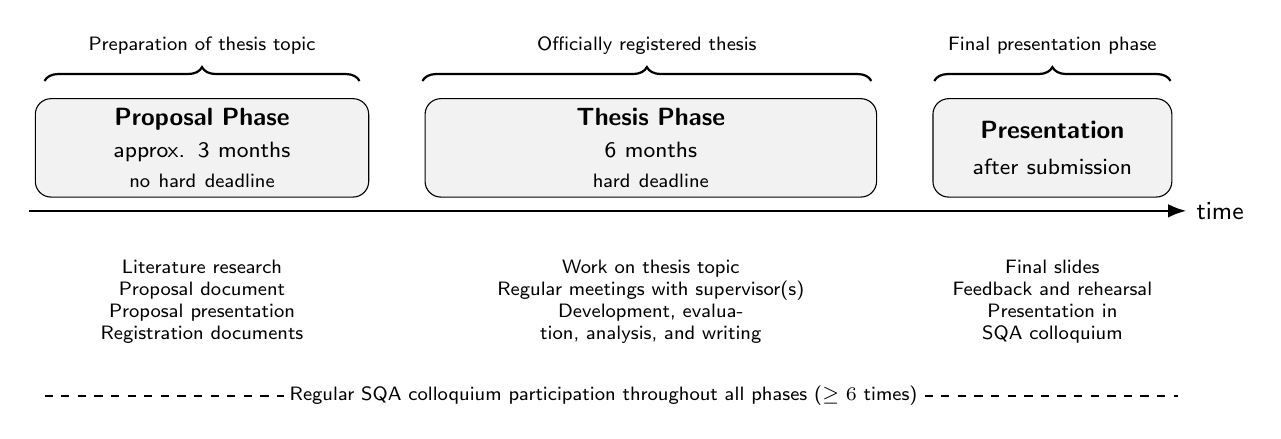
\begin{tikzpicture}[
    font=\small,
    >=Latex,
    phase/.style={
        draw,
        rounded corners=2mm,
        minimum height=1.25cm,
        align=center,
        fill=gray!10
    },
    milestone/.style={
        draw,
        circle,
        minimum size=7mm,
        fill=white,
        align=center,
        font=\scriptsize
    },
    note/.style={
        align=center,
        font=\scriptsize
    },
    activity/.style={
        align=center,
        font=\scriptsize,
        text width=3.2cm
    }
]

% Timeline axis
\draw[->, thick] (0,0) -- (14.7,0) node[right] {time};

% Phases
\node[phase, text width=4.0cm] (proposal) at (2.2,0.8)
{\textbf{Proposal Phase}\\[0.2em]
\footnotesize approx. 3 months\\
\scriptsize no hard deadline};

\node[phase, text width=5.5cm] (thesis) at (7.9,0.8)
{\textbf{Thesis Phase}\\[0.2em]
\footnotesize 6 months\\
\scriptsize hard deadline};

\node[phase, text width=2.8cm] (presentation) at (13.0,0.8)
{\textbf{Presentation}\\[0.2em]
\footnotesize after submission};

% Phase duration brackets
\draw[decorate, decoration={brace, amplitude=5pt}, thick]
    (0.2,1.65) -- (4.2,1.65)
    node[midway, yshift=0.45cm, note] {Preparation of thesis topic};

\draw[decorate, decoration={brace, amplitude=5pt}, thick]
    (5.0,1.65) -- (10.7,1.65)
    node[midway, yshift=0.45cm, note] {Officially registered thesis};

\draw[decorate, decoration={brace, amplitude=5pt}, thick]
    (11.5,1.65) -- (14.5,1.65)
    node[midway, yshift=0.45cm, note] {Final presentation phase};

% Milestones on timeline
%\node[milestone] (start) at (0.2,0) {};
%\node[note, below=0.25cm of start] {Start};

%\node[milestone] (proptalk) at (4.2,0) {};
%\node[note, below=0.25cm of proptalk] {Proposal\\talk};

%\node[milestone] (registration) at (5.0,0) {};
%\node[note, below=0.25cm of registration] {Thesis\\registration};

%\node[milestone] (submission) at (10.7,0) {};
%\node[note, below=0.25cm of submission] {Submission\\deadline};

%\node[milestone] (finaltalk) at (12.4,0) {};
%\node[note, below=0.25cm of finaltalk] {Final\\presentation};

% Activities below phases
\node[activity] at (2.2,-1.15)
{Literature research\\
Proposal document\\
Proposal presentation\\
Registration documents};

\node[activity, text width=4.6cm] at (7.9,-1.15)
{Work on thesis topic\\
Regular meetings with supervisor(s)\\
Development, evaluation, analysis, and writing};

\node[activity] at (13.0,-1.15)
{Final slides\\
Feedback and rehearsal\\
Presentation in SQA colloquium};

% Colloquium participation line
\draw[thick, dashed] (0.2,-2.35) -- (14.6,-2.35);
\node[align=center, font=\scriptsize, fill=white, inner sep=2pt] at (7.3,-2.35)
{Regular SQA colloquium participation throughout all phases ($\geq6$ times)};

% Colloquium markers
%\foreach \x in {1.0,2.0,3.0,5.2,6.2,7.2,8.2,9.2,11.2}
%    \draw[fill=white] (\x,-2.35) circle (1.8pt);

% Highlight proposal and final talks as colloquium events
%\draw[thick] (4.2,0) -- (4.2,-2.35);
%\draw[thick] (12.4,0) -- (12.4,-2.35);

\end{tikzpicture}
\caption{Overview of the thesis process in the ISTE/SQA group.}
\label{fig:thesis-process}
\end{figure}

\section{Grading Criteria and Schema}
The examiner(s) grade the thesis according to the common 0.3-step scale between 1.0 and 5.0 (failed).
The final grade is based on the following criteria and approximate proportions.
If a thesis or project is formally ungraded, it is still expected to satisfy the quality standards of a graded thesis.

\begin{center}
    \begin{tabular}{|p{10.5cm}|p{4cm}|}
    \toprule
    \textbf{Criterion} & \textbf{Approx. Proportion}  \\ \midrule
    Course of the thesis (self-organization, timeliness, communication, independence, ...) & 10\% \\ \hline
    Concept and implementation (research design, solution approach, realization, evaluation) & 20\% \\ \hline
    Thesis document (structure, presentation quality, completeness, scientific quality, discussion) & 40\% \\ \hline
    Final presentation (quality of slides, structure, talk, discussion) & 20-30\% \\ \hline
    Other criterias & 0-10\% \\ \bottomrule
    \end{tabular}
\end{center}


% \section{Prop\"adeutikum for Bachelor's Theses}
% In the new examination regulations, Bachelor students may have to complete a \emph{Prop\"adeutikum} worth 6 ECTS before the actual Bachelor's thesis.

% At ISTE/SQA, the Prop\"adeutikum is used as a preparatory phase for the Bachelor's thesis.
% The main goal is to conduct a systematic literature research and to prepare the foundations for the thesis.
% The work conducted in the Prop\"adeutikum is graded according to the applicable examination regulations.

% The expected output of the Prop\"adeutikum is the proposal document and presentation (see Section~\ref{sec:proposal}.

% \subsection*{Propädeutikum Checklist}

% \begin{longtable}{|p{12.5cm}|p{1.5cm}|}
% \hline
% \textbf{Checklist Item} & \textbf{Done} \\
% \hline
% I have clarified the topic, scope, and expected outcome of the Propädeutikum with my supervisor. & \checkbox \\
% \hline
% I have conducted a literature research covering relevant foundations and related work. & \checkbox \\
% \hline
% I have documented the literature research in the proposal document. & \checkbox \\
% \hline
% I have identified the research gap, practical problem, or scientific motivation for the thesis. & \checkbox \\
% \hline
% I have prepared the proposal document as the main written output of the Propädeutikum. & \checkbox \\
% \hline
% I have prepared the proposal presentation as the oral output of the Propädeutikum. & \checkbox \\
% \hline
% I have submitted the required Propädeutikum outputs according to the instructions of my supervisor and examiner. & \checkbox \\
% \hline
% \end{longtable}
\section{\LaTeX\ Template}
For all the documents that the student submits, ISTE/SQA provides various \LaTeX\ templates in GitHub\footnote{\url{https://github.com/ISTE-SQA}}.

\section{Proposal Phase}\label{sec:proposal}
Each student writing a Bachelor's or Master's thesis must complete a proposal phase before officially registering and starting the thesis.
The proposal phase prepares the actual thesis work and ensures that the topic, motivation, research context, planned approach, and schedule are sufficiently clear.

For students who have a \textit{Prop\"adeutikum} according to their examination regulations, the Prop\"adeutikum corresponds to the proposal phase.
In this case, the proposal phase (presentation + document) is graded.

The proposal phase is conducted in close interaction with the supervisor(s). After successful completion of the proposal phase, the student can proceed with the official thesis registration, subject to the applicable examination regulations and approval by the examiner.

\subsection{Proposal Document}
The proposal document describes the planned thesis topic.
It must explain the problem addressed by the thesis, outline the envisioned approach, consider relevant foundations and related work, and provide a realistic work plan and schedule.

\subsubsection*{Checklist}
\begin{checklisttable}{Checklist for the proposal document}{tab:checklist-proposal-document}

\checkgroup{Content: The proposal document contains...}
\checkitem{...context and motivation of the thesis topic}
\checkitem{...a clear problem statement}
\checkitem{...the goal of the thesis.}
\checkitem{...the relevant foundations}
\checkitem{...related work and the state of the art.}
\checkitem{...research gap, practical problem, or scientific motivation.}
\checkitem{...planned research question(s), objective(s), or hypotheses.}
\checkitem{...planned research method, approach, or implementation strategy.}
\checkitem{...a realistic work plan and schedule.}

\checksep
\checkgroup{Feedback and Acceptance}
\checkitem{I have sent the proposal to my supervisor for feedback.}
\checkitem{I have revised the proposal based on feedback.}
\checkitem{The proposal has been accepted by the supervisor(s).}
\end{checklisttable}

\subsection{Proposal Presentation}
In the proposal talk, the student presents the planned thesis topic in the SQA colloquium.
The proposal talk covers the contents of the proposal document and aims to obtain feedback from the examiner(s), members of the SQA group, and other students attending the colloquium.

A 30-minute slot is allocated for each proposal presentation. A \important{maximum of 15 minutes} must be used or the talk. The remaining 15 minutes are reserved for discussion. \important{The slides and the talk should be in English.}

\begin{checklisttable}{Checklist for the proposal presentation}{tab:proposal-presentation}

\checkgroup{Content: The proposal presentation...}
\checkitem{...includes a concise motivation of the problem.}
\checkitem{...includes a clear problem statement.}
\checkitem{...states the goal of the thesis.}
\checkitem{...explains the relation to the state of the art.}
\checkitem{...presents the planned approach, method, or research design.}
\checkitem{...includes a work plan and schedule.}

\checksep
\checkgroup{Preparation and Feedback}
\checkitem{I have considered the SQA guidelines on how to give a good scientific talk.}
\checkitem{I have sent the slides to my supervisor(s) and rehearsed my presentation.}
\checkitem{I have uploaded the proposal and the slides to ILIAS.}
\checkitem{I have received confirmation that I passed the proposal phase.}
\end{checklisttable}

\subsection{Prop\"adeutikum}
In the new examination regulations, some Bachelor students have to complete a Prop\"adeutikum worth 6 ECTS before the actual Bachelor's thesis.

At ISTE/SQA, the Prop\"adeutikum is the graded version of the proposal phase. It consists of the proposal document and the proposal presentation.
The main purpose of the Prop\"adeutikum is to conduct and document the preparatory work for the Bachelor's thesis, especially the literature research on foundations and related work.

The Prop\"adeutikum does not introduce a separate additional phase beyond the proposal phase.
Instead, it means that the proposal phase is formally graded.

\section{Registration Documents}
The student must officially register the thesis after the proposal phase has been passed.

Additional information about the process for Bachelor's and Master's thesis can be further found on the faculty website\footnote{\url{https://www.f05.uni-stuttgart.de/informatik/studierende/abschlussarbeiten/}}.

\begin{checklisttable}{Checklist for Registration}{tab:registration}

\checkgroup{Preparation of Documents}
\checkitem{I have prepared the registration form via C@mpus.}
\checkitem{I have prepared the contract.}
\checkitem{I have prepared the license agreement.}
\checkitem{I have prepared the request for writing the thesis in English, if required.}
\checkitem{I have prepared the one-page topic description, including the name(s) of the examiner and supervisor(s).}
\addlinespace[0.5em]
\checkgroup{Approval}

\checkitem{The registration documents and topic description have been approved by the supervisor(s).}

\addlinespace[0.5em]
\checkgroup{Submission}

\checkitem{I have submitted the registration documents to the SQA secretary and examination office.}

\end{checklisttable}

\section{Thesis}
The thesis phase is the main phase o the thesis process.
During this phase, the student conducts the actual thesis work, writes the thesis document, and prepares the final presentation.

The thesis work must follow scientific standards and good scientific practice.
The student is responsible for the correctness, originality, tracability, and scientific quality of the submitted work.
This also applies if AI tools are used during the thesis.

\subsection{Use of AI Tools}
Students are allowed to use AI tools in accordance with the AI guideline of the University of Stuttgart\footnote{German version: \url{https://www.student.uni-stuttgart.de/digital-services/ki-fuer-studierende/}}\footnote{English version: \url{https://www.student.uni-stuttgart.de/en/digital-services/ai-for-students/}}.

AI tools may be used as supporting tools, for example for brainstorming, language improvement, structuring, summarization, programming support, or other thesis-related assistance.
However, the use of AI tools must not replace the student's own personal engagement, independent thinking, scientific reasoning, or responsibility for good scientific practice.

The student remains fully responsible for all submitted content, including correctness, originality, citations, references, argumentation, and compliance with scientific ethics.

\subsubsection*{Documentation of AI Tool Usage}
If AI tools are used during the thesis, the thesis document must contain an appendix titled \emph{Usage of AI Tools}.
In this appendix, the student must document the use of AI tools.
For each relevant use, the documentation must include at least:
\begin{itemize}
    \item the AI tool that was used,
    \item where it was used in the thesis or thesis process,
    \item the prompt or input given to the AI tool,
    \item the purpose of using the tool,
    \item how the AI output was checked, adapted, or used by the student.
\end{itemize}

The ISTE/SQA \LaTeX\ thesis template already provides a format for this appendix.

Students must not enter confidential, sensitive, personal, unpublished, or legally protected data into external AI tools unless this is explicitly permitted and legally safe.
When possible, students should prefer AI tools provided or recommended by the University of Stuttgart.

\subsection{Document}
The thesis document provides a comprehensive scientific report about the conducted thesis project.
Students are strongly encouraged to have regular meetings with the supervisor(s) and to ask for feedback early enough.

The thesis document must follow scientific standards. It must introduce the topic, explain relevant concepts and foundations, discuss related work and the state of the art, clearly state the addressed problem, explain the chosen approach, present the obtained results, and discuss the results including limitations and threats to validity.

\begin{checklisttable}{Checklist for the thesis document}{tab:thesis-document-checklist}
\checkgroup{Content}
\checkitem{The thesis includes an introduction with context, motivation, and a clear problem statement.}
\checkitem{The thesis covers all relevant foundations.}
\checkitem{The thesis covers related work and the state of the art.}
\checkitem{The thesis explains how the addressed problem differs from or extends existing work.}
\checkitem{The thesis describes the research question(s), objective(s), or hypotheses.}
\checkitem{The thesis describes the applied research method(s), design decisions, implementation, or evaluation approach.}
\checkitem{The thesis presents the obtained results clearly and systematically.}
\checkitem{The thesis discusses the results rationally and critically.}
\checkitem{The thesis covers limitations and threats to validity.}

\addlinespace[0.5em]
\checkgroup{AI Usage}
\checkitem{I have read and considered the University of Stuttgart guideline on the use of AI tools by students.}
\checkitem{I have used AI tools only as support and not as a replacement for my own scientific work, reasoning, and responsibility.}
\checkitem{I have checked the correctness, relevance, and scientific validity of AI-generated or AI-supported outputs.}
\checkitem{If I used AI tools, the thesis includes an appendix titled \emph{Usage of AI Tools}, documenting the tool, location of use, prompt, purpose, and how the output was checked or adapted.}

\addlinespace[0.5em]
\checkgroup{Preparation and Feedback}
\checkitem{I have asked my supervisor(s) for feedback early enough.}
\checkitem{At least 14 days before the submission date, I have clarified whether printed copies and thesis covers are required.}

\end{checklisttable}

\subsection{Final Presentation}
In the final presentation, the student presents the outcomes of the thesis in the SQA colloquium.
The presentation covers the contents of the thesis document and focuses on the main motivation, approach, results, discussion, and lessons learned.

A 30-minute slot is allocated for each final presentation.
A \important{maximum of 20 minutes} must be used for the talk.
The remaining 10 minutes are reserved for discussion.
The slides and the talk should be in English.

\begin{checklisttable}{Checklist for the final presentation}{tab:final-presentation-checklist}

\checkgroup{Content of the Presentation}
\checkitem{The final presentation includes a concise motivation of the problem, preferably using an example.}
\checkitem{The final presentation includes a clear problem statement.}
\checkitem{The final presentation states the goal of the thesis.}
\checkitem{The final presentation gives an overview of the conducted work and applied methods.}
\checkitem{The final presentation gives an in-depth presentation of selected results.}
\checkitem{The final presentation discusses limitations and threats to validity.}
\checkitem{The final presentation gives pointers to possible future work.}

\addlinespace[0.5em]
\checkgroup{Preparation and Feedback}

\checkitem{I have considered the SQA guidelines on how to give a good scientific presentation.}
\checkitem{I have sent the slides to my supervisor for feedback.}
\checkitem{I have discussed the slides with my supervisor, preferably including a rehearsal.}
\checkitem{The talk is ready for the colloquium.}

\end{checklisttable}

% \begin{longtable}{|p{12.5cm}|p{1.5cm}|}
% \hline
% \textbf{Checklist Item} & \textbf{Done} \\ \hline
% The final presentation includes a concise motivation of the problem, preferably using an example. & \checkbox \\ \hline
% The final presentation includes a clear problem statement. & \checkbox \\ \hline
% The final presentation states the goal of the thesis. & \checkbox \\ \hline
% The final presentation gives an overview of the conducted work and applied methods. & \checkbox \\ \hline
% The final presentation gives an in-depth presentation of selected results. & \checkbox \\ \hline
% The final presentation discusses limitations and threats to validity. & \checkbox \\ \hline
% The final presentation gives pointers to possible future work. & \checkbox \\ \hline
% I have considered the SQA guidelines on how to give a good scientific presentation. & \checkbox \\ \hline \hline
% I have sent the slides to my supervisor for feedback. & \checkbox \\ \hline 
% I have discussed the slides with my supervisor, preferably including a rehearsal. & \checkbox \\ \hline
% The talk is ready for the colloquium & \checkbox \\ \hline
% \end{longtable}

\section{Colloquium Participation}
The SQA colloquium is a regular seminar in which students present the proposal and the results of their theses.
Each student must attend the colloquium \important{at least six times} (including the colloquiums in which the students presents).
A member of the SQA group confirms the participation.

\section*{AI Usage Notice.}
This document was revised with support from ChatGPT. The tool was used for language improvements, for generating a TikZ-based process overview, and for improving the visual structure of checklist tables. All AI-supported suggestions were reviewed, selected, and adapted by the authors of this document.

\end{document}
